% Created by tikzDevice version 0.12.3.1 on 2022-08-16 16:14:03
% !TEX encoding = UTF-8 Unicode
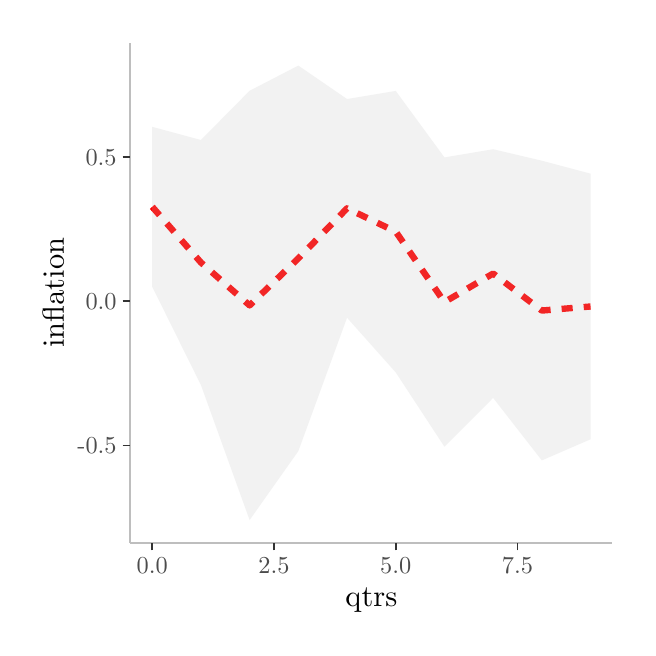
\begin{tikzpicture}[x=1pt,y=1pt]
\definecolor{fillColor}{RGB}{255,255,255}
\path[use as bounding box,fill=fillColor,fill opacity=0.00] (0,0) rectangle (216.81,216.81);
\begin{scope}
\path[clip] (  0.00,  0.00) rectangle (216.81,216.81);
\definecolor{drawColor}{RGB}{255,255,255}
\definecolor{fillColor}{RGB}{255,255,255}

\path[draw=drawColor,line width= 0.6pt,line join=round,line cap=round,fill=fillColor] (  0.00,  0.00) rectangle (216.81,216.81);
\end{scope}
\begin{scope}
\path[clip] ( 37.09, 30.69) rectangle (211.31,211.31);
\definecolor{drawColor}{RGB}{255,255,255}

\path[draw=drawColor,line width= 0.6pt,line join=round] ( 37.09, 65.83) --
	(211.31, 65.83);

\path[draw=drawColor,line width= 0.6pt,line join=round] ( 37.09,117.95) --
	(211.31,117.95);

\path[draw=drawColor,line width= 0.6pt,line join=round] ( 37.09,170.06) --
	(211.31,170.06);

\path[draw=drawColor,line width= 0.6pt,line join=round] ( 45.01, 30.69) --
	( 45.01,211.31);

\path[draw=drawColor,line width= 0.6pt,line join=round] ( 89.00, 30.69) --
	( 89.00,211.31);

\path[draw=drawColor,line width= 0.6pt,line join=round] (133.00, 30.69) --
	(133.00,211.31);

\path[draw=drawColor,line width= 0.6pt,line join=round] (176.99, 30.69) --
	(176.99,211.31);
\definecolor{drawColor}{RGB}{255,0,0}

\path[draw=drawColor,line width= 2.3pt,dash pattern=on 4pt off 4pt ,line join=round] ( 45.01,152.08) --
	( 62.61,131.95) --
	( 80.20,116.45) --
	( 97.80,133.45) --
	(115.40,151.52) --
	(133.00,143.10) --
	(150.60,117.65) --
	(168.19,127.96) --
	(185.79,114.59) --
	(203.39,116.06);
\definecolor{fillColor}{RGB}{190,190,190}

\path[fill=fillColor,fill opacity=0.20] ( 45.01,180.97) --
	( 62.61,176.21) --
	( 80.20,194.00) --
	( 97.80,203.10) --
	(115.40,191.02) --
	(133.00,193.94) --
	(150.60,169.92) --
	(168.19,172.88) --
	(185.79,168.73) --
	(203.39,164.05) --
	(203.39, 68.08) --
	(185.79, 60.45) --
	(168.19, 83.04) --
	(150.60, 65.39) --
	(133.00, 92.25) --
	(115.40,112.02) --
	( 97.80, 63.81) --
	( 80.20, 38.90) --
	( 62.61, 87.69) --
	( 45.01,123.19) --
	cycle;

\path[] ( 45.01,180.97) --
	( 62.61,176.21) --
	( 80.20,194.00) --
	( 97.80,203.10) --
	(115.40,191.02) --
	(133.00,193.94) --
	(150.60,169.92) --
	(168.19,172.88) --
	(185.79,168.73) --
	(203.39,164.05);

\path[] (203.39, 68.08) --
	(185.79, 60.45) --
	(168.19, 83.04) --
	(150.60, 65.39) --
	(133.00, 92.25) --
	(115.40,112.02) --
	( 97.80, 63.81) --
	( 80.20, 38.90) --
	( 62.61, 87.69) --
	( 45.01,123.19);
\end{scope}
\begin{scope}
\path[clip] (  0.00,  0.00) rectangle (216.81,216.81);
\definecolor{drawColor}{RGB}{190,190,190}

\path[draw=drawColor,line width= 0.6pt,line join=round] ( 37.09, 30.69) --
	( 37.09,211.31);
\end{scope}
\begin{scope}
\path[clip] (  0.00,  0.00) rectangle (216.81,216.81);
\definecolor{drawColor}{gray}{0.30}

\node[text=drawColor,anchor=base east,inner sep=0pt, outer sep=0pt, scale=  0.88] at ( 32.14, 62.80) {-0.5};

\node[text=drawColor,anchor=base east,inner sep=0pt, outer sep=0pt, scale=  0.88] at ( 32.14,114.92) {0.0};

\node[text=drawColor,anchor=base east,inner sep=0pt, outer sep=0pt, scale=  0.88] at ( 32.14,167.03) {0.5};
\end{scope}
\begin{scope}
\path[clip] (  0.00,  0.00) rectangle (216.81,216.81);
\definecolor{drawColor}{gray}{0.20}

\path[draw=drawColor,line width= 0.6pt,line join=round] ( 34.34, 65.83) --
	( 37.09, 65.83);

\path[draw=drawColor,line width= 0.6pt,line join=round] ( 34.34,117.95) --
	( 37.09,117.95);

\path[draw=drawColor,line width= 0.6pt,line join=round] ( 34.34,170.06) --
	( 37.09,170.06);
\end{scope}
\begin{scope}
\path[clip] (  0.00,  0.00) rectangle (216.81,216.81);
\definecolor{drawColor}{RGB}{190,190,190}

\path[draw=drawColor,line width= 0.6pt,line join=round] ( 37.09, 30.69) --
	(211.31, 30.69);
\end{scope}
\begin{scope}
\path[clip] (  0.00,  0.00) rectangle (216.81,216.81);
\definecolor{drawColor}{gray}{0.20}

\path[draw=drawColor,line width= 0.6pt,line join=round] ( 45.01, 27.94) --
	( 45.01, 30.69);

\path[draw=drawColor,line width= 0.6pt,line join=round] ( 89.00, 27.94) --
	( 89.00, 30.69);

\path[draw=drawColor,line width= 0.6pt,line join=round] (133.00, 27.94) --
	(133.00, 30.69);

\path[draw=drawColor,line width= 0.6pt,line join=round] (176.99, 27.94) --
	(176.99, 30.69);
\end{scope}
\begin{scope}
\path[clip] (  0.00,  0.00) rectangle (216.81,216.81);
\definecolor{drawColor}{gray}{0.30}

\node[text=drawColor,anchor=base,inner sep=0pt, outer sep=0pt, scale=  0.88] at ( 45.01, 19.68) {0.0};

\node[text=drawColor,anchor=base,inner sep=0pt, outer sep=0pt, scale=  0.88] at ( 89.00, 19.68) {2.5};

\node[text=drawColor,anchor=base,inner sep=0pt, outer sep=0pt, scale=  0.88] at (133.00, 19.68) {5.0};

\node[text=drawColor,anchor=base,inner sep=0pt, outer sep=0pt, scale=  0.88] at (176.99, 19.68) {7.5};
\end{scope}
\begin{scope}
\path[clip] (  0.00,  0.00) rectangle (216.81,216.81);
\definecolor{drawColor}{RGB}{0,0,0}

\node[text=drawColor,anchor=base,inner sep=0pt, outer sep=0pt, scale=  1.10] at (124.20,  7.64) {qtrs};
\end{scope}
\begin{scope}
\path[clip] (  0.00,  0.00) rectangle (216.81,216.81);
\definecolor{drawColor}{RGB}{0,0,0}

\node[text=drawColor,rotate= 90.00,anchor=base,inner sep=0pt, outer sep=0pt, scale=  1.10] at ( 13.08,121.00) {inflation};
\end{scope}
\end{tikzpicture}
